\section{根付き全域森問題}
本節では本研究で取り扱う根付き全域森について説明する.
前節で述べたように,供給経路に関するトポロジ制約を満たす
配電網構成は,変電所を根とする根付き全域森に対応する.
この根付き全域森を探索するグラフ問題を\textbf{根付き全域森問題}と呼ぶ.

根付き全域森は以下のように定義される.\cite{Minato:dnet:netuki}
\newline
\textbf{定義}~~グラフ$G=(V,E)$と根$R$が入力として与えられたとする.
このとき,$G$上の根付き全域森とは,以下の2つの制約を満たす$G$の部分グラフ
$G'=(V,E'), E' \subseteq E$ である.
\begin{enumerate}
 \item $G'$はサイクルを持たない.\textbf{(非閉路制約)}
 \item $G'$の各連結成分は,ちょうど1つの根を含む.\textbf{(根付き連結制約)}
\end{enumerate}
図\ref{fig:dnetgraph}における根付き全域森の例を図\ref{fig:netuki}に示す.

%%%%%%%%%%%%%%%%%%%%%%%%%
\begin{figure}[htbp]
 %
 %\begin{minipage}{0.5\hsize}
  \centering
  \scalebox{0.8}{%%%%%%%%%%%%%%%%%%%%%%%%%%%%%%%%%%%%%%%%%%%%%%%%%%
% 根付き全域森 (第2章で使う)
%%%%%%%%%%%%%%%%%%%%%%%%%%%%%%%%%%%%%%%%%%%%%%%%%%

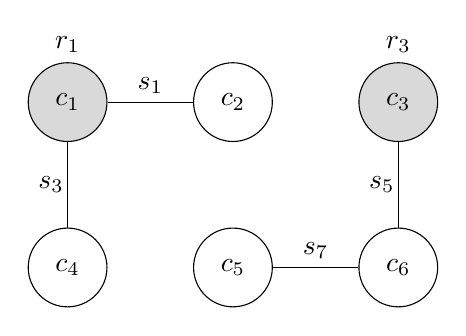
\begin{tikzpicture}[x=1.5cm,y=1.5cm,scale=0.7]

 % 設定
 \tikzset{root/.style={circle,draw=black,fill=gray!30,minimum size=1cm}}
 \tikzset{node/.style={circle,draw=black,minimum size=1cm}}
 
 % 補助線
 % \draw [help lines,blue,step=2cm] (-3,0) grid (3,-3);

 % root %
 \node[root] at (-2,0) (1){$c_1$};
 \node[above=0.5cm] at (1) {$r_1$};
 \node[root] at (2,0) (3){$c_3$};
 \node[above=0.5cm] at (3) {$r_3$};

 % node %
 \node[node] at (0,0) (2){$c_2$};
 \node[node] at (-2,-2) (4){$c_4$};
 \node[node] at (0,-2) (5){$c_5$};
 \node[node] at (2,-2) (6){$c_6$};

 % 繋がっていない辺は破線
 %\foreach \u / \v in {2/3, 2/5, 4/5}
 %\draw [dashed] (\u) -- (\v);
 % 繋がってる辺は実線
 \foreach \u / \v in {1/2, 1/4, 3/6, 5/6}
 \draw (\u) -- (\v);

 % スイッチ switch %
 \node at (-1,0.2) {$s_1$};
 %\node at (1,0.2) {$s_2$};
 \node at (-2.2,-1) {$s_3$};
 %\node at (-0.2,-1) {$s_4$};
 \node at (1.8,-1) {$s_5$};
 %\node at (-1,-1.8) {$s_6$};
 \node at (1,-1.8) {$s_7$};
 %

\end{tikzpicture}

%%%%%%%%%%%%%%%%%%%%%%%%%%%%%%%%%%%%%%%%%%%%%%%%%%%%%%%%%%
%%% Local Variables:
%%% mode: japanese-latex
%%% TeX-master: paper.tex
%%% End:
}
 %\end{minipage}
 %
% \begin{minipage}{0.5\hsize}
 \mbox{}\\ \mbox{}\\
  \centering
  \scalebox{0.8}{%%%%%%%%%%%%%%%%%%%%%%%%%%%%%%%%%%%%%%%%%%%%%%%%%%
% 根付き全域森 (第2章で使う)
%%%%%%%%%%%%%%%%%%%%%%%%%%%%%%%%%%%%%%%%%%%%%%%%%%

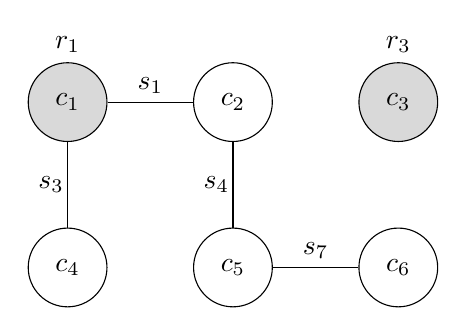
\begin{tikzpicture}[x=1.5cm,y=1.5cm,scale=0.7]

 % 設定
 \tikzset{root/.style={circle,draw=black,fill=gray!30,minimum size=1cm}}
 \tikzset{node/.style={circle,draw=black,minimum size=1cm}}
 
 % 補助線
 % \draw [help lines,blue,step=2cm] (-3,0) grid (3,-3);

 % root %
 \node[root] at (-2,0) (1){$c_1$};
 \node[above=0.5cm] at (1) {$r_1$};
 \node[root] at (2,0) (3){$c_3$};
 \node[above=0.5cm] at (3) {$r_3$};

 % node %
 \node[node] at (0,0) (2){$c_2$};
 \node[node] at (-2,-2) (4){$c_4$};
 \node[node] at (0,-2) (5){$c_5$};
 \node[node] at (2,-2) (6){$c_6$};

 % 繋がっていない辺は破線
 %\foreach \u / \v in {2/3, 2/5, 4/5}
 %\draw [dashed] (\u) -- (\v);
 % 繋がってる辺は実線
 \foreach \u / \v in {1/2, 1/4, 2/5, 5/6}
 \draw (\u) -- (\v);

 % スイッチ switch %
 \node at (-1,0.2) {$s_1$};
 %\node at (1,0.2) {$s_2$};
 \node at (-2.2,-1) {$s_3$};
 \node at (-0.2,-1) {$s_4$};
 %\node at (1.8,-1) {$s_5$};
 %\node at (-1,-1.8) {$s_6$};
 \node at (1,-1.8) {$s_7$};
 %

\end{tikzpicture}

%%%%%%%%%%%%%%%%%%%%%%%%%%%%%%%%%%%%%%%%%%%%%%%%%%%%%%%%%%
%%% Local Variables:
%%% mode: japanese-latex
%%% TeX-master: paper.tex
%%% End:
}
% \end{minipage}
 %
 \caption{根付き全域森の例}
 \label{fig:netuki}
\end{figure}
%%%%%%%%%%%%%%%%%%%%%%%%%

% グラフの説明
図\ref{fig:netuki}のように根付き全域森は1つの入力グラフに対し,
複数存在する.根付き全域森は,非連結であることを許すが,
各連結成分が必ずちょうど1つの根を持つ木構造を形成することで,
非閉路制約と根付き連結制約を満たす.図\ref{fig:netuki}(上)は,
図\ref{fig:dnet}で表した実行可能解をグラフ表現に置き換えたものである.
また,解の一部には図\ref{fig:netuki}(下)のように,ある連結成分が根のみ
の場合もある.
